\documentclass[11pt]{article}
\usepackage{amssymb}
\usepackage{amsthm}
\usepackage{enumitem}
\usepackage{amsmath, physics}
\usepackage{bm}
\usepackage{adjustbox}
\usepackage{mathrsfs}
\usepackage{graphicx}
\usepackage{siunitx}
\usepackage[mathscr]{euscript}

\title{\textbf{Solved selected problems of Classical Electrodynamics - Hans Ohanian}}
\author{Franco Zacco}
\date{}

\addtolength{\topmargin}{-3cm}
\addtolength{\textheight}{3cm}

\newcommand{\N}{\mathbb{N}}
\newcommand{\Z}{\mathbb{Z}}
\newcommand{\Q}{\mathbb{Q}}
\newcommand{\R}{\mathbb{R}}
\newcommand{\diam}{\text{diam}}
\newcommand{\cl}{\text{cl}}
\newcommand{\bdry}{\text{bdry}}
\newcommand{\inter}{\text{int}}
\newcommand{\uvi}{\bm{i}}
\newcommand{\uvj}{\bm{j}}
\newcommand{\uvk}{\bm{k}}
\newcommand{\hatx}{\bm{\hat{x}}}
\newcommand{\haty}{\bm{\hat{y}}}
\newcommand{\hatz}{\bm{\hat{z}}}
\newcommand{\hatrho}{\bm{\hat{\rho}}}
\newcommand{\hatphi}{\bm{\hat{\phi}}}
\newcommand{\hatr}{\bm{\hat{r}}}
\newcommand{\hattheta}{\bm{\hat{\theta}}}
\newcommand\numberthis{\addtocounter{equation}{1}\tag{\theequation}}

\theoremstyle{definition}
\newtheorem*{solution*}{Solution}
\renewcommand*{\proofname}{\bf{Solution}}

\begin{document}
\maketitle
\thispagestyle{empty}

\section*{Chapter 2 - Electrostatics}

\subsection*{Problems}
\begin{proof}{\textbf{1.}}
    Let us suppose we have a proton and an electron at a distance $r$
    then the magnitude of the gravitational force exerted on the proton
    by the electron is 
    \begin{align*}
        F_{\text{grav}} &= G\frac{m_em_p}{r^2}\\
        &= 6.674 \times 10^{-8}~\frac{dyne \cdot cm^2}{g^2}
        \cdot\frac{9.10938\times 10^{-28}~g
        \cdot 1.67262 \times 10^{-24}~g}{r^2}
    \end{align*}
    On the other hand, the magnitude of the electric force exerted on the
    proton by the electron is
    \begin{align*}
        F_{\text{electric}} &= \frac{|q_e q_p|}{r^2}\\
        &= \frac{(4.803207\times 10^{-10}~esu)^2}{r^2}
    \end{align*}
    So the ratio between the gravitational and the electrical force is
    \begin{align*}
        \frac{F_{\text{electric}}}{F_{\text{grav}}}
        = \frac{2.307079 \times 10^{-19}}{1.01688\times 10^{-58}}
        = 2.26876 \times 10^{39}
    \end{align*}
\end{proof}
\cleardoublepage
\begin{proof}{\textbf{4.}}
    Let us consider a system that looks like the following
    \begin{center}
        \includegraphics*[scale=0.3]{ch2-4.png}
    \end{center}
    We know the rods carry a uniformly distributed charge $Q$ so the charge
    per unit of length is $Q/L$ then if we consider a small piece of rod $dx'$
    it will carry a charge of $(Q/L)dx'$ so at a distance of $x' + x + d$ this
    small charge contributes an electric field of magnitude
    \begin{align*}
        dE = \frac{Q}{L} \frac{dx}{(x'+ x + d)^2}
    \end{align*}
    So by integration, we have that
    \begin{align*}
        E &= \int_0^L \frac{Q}{L} \frac{dx'}{(x'+ x +d)^2}\\
        &= \frac{Q}{L} \bigg[-\frac{1}{x' + x + d}\bigg]_0^L\\
        &= \frac{Q}{L} \bigg[-\frac{1}{L + x + d} + \frac{1}{x + d}\bigg]\\
        &= \frac{Q}{L} \frac{L}{(x + d)(x + d + L)}\\
        &= \frac{Q}{(x + d)(x + d + L)}
    \end{align*}
    Therefore the force on a small charge $(Q/L)dx$ on the other rod is
    $(Q/L)E~dx$ so again by integration we have that
    \begin{align*}
        F &= \int_0^L \frac{Q}{L}E~dx\\
        &= \int_0^L \frac{Q^2}{L(x + d)(x + d + L)}~dx\\
        &= \frac{Q^2}{L}\int_0^L \frac{1}{(x + d)(x + d + L)}~dx\\
        &= \frac{Q^2}{L}\bigg[\frac{\log(x + d) - \log(x + d + L)}{L}\bigg]_0^L\\
        &= \frac{Q^2}{L^2}\bigg[
            \log(L + d) - \log(d + 2L) - \log(d) + \log(d + L)
        \bigg]\\
        &= \frac{Q^2}{L^2}\bigg[
            2\log(L + d) - \log(d + 2L) - \log(d)
        \bigg]
    \end{align*}
\end{proof}
\begin{proof}{\textbf{6.}}
    Let us consider a system that looks like the following
    \begin{center}
        \includegraphics*[scale=0.35]{ch2-6.png}
    \end{center}
    Let us consider a small piece of area in polar coordinates $r'dr'd\phi'$
    then this small piece carries a charge $\sigma r'dr'd\phi'$ where 
    $\sigma =0$ if $r' < R_1$. Then at a height $z$ above the annulus
    this charge contributes an electric field of magnitude
    \begin{align*}
        dE = \frac{\sigma r' dr' d\phi'}{z^2 + r'^2}
    \end{align*}
    This electric field has both a vertical and a horizontal component.
    In view of the symmetry of the charge distribution, the horizontal
    components cancel upon integration. Hence we need to consider only
    the vertical components
    \begin{align*}
        dE_z &= \cos\theta\frac{\sigma r' dr' d\phi'}{z^2 + r'^2}\\
        &= \frac{z}{\sqrt{z^2 + r'^2}}\frac{\sigma r' dr' d\phi'}{z^2 + r'^2}\\
        &= \frac{\sigma zr' dr' d\phi'}{(z^2 + r'^2)^{3/2}}
    \end{align*}
    Now by integration we have that
    \begin{align*}
        E &= \sigma \int_{R_1}^{R_2} \int_{0}^{2\pi}
        \frac{ zr' dr' d\phi'}{(z^2 + r'^2)^{3/2}}\\
        E &= 2\pi \sigma \int_{R_1}^{R_2}
        \frac{ zr' dr'}{(z^2 + r'^2)^{3/2}}\\
        E &= 2\pi \sigma \bigg[-\frac{z}{\sqrt{z^2 + r'^2}}\bigg]_{R_1}^{R_2}\\
        E &= 2\pi \sigma z \bigg[\frac{1}{\sqrt{z^2 + R_1^2}}
        -\frac{1}{\sqrt{z^2 + R_2^2}}\bigg]
    \end{align*}

\end{proof}
\begin{proof}{\textbf{7.}}
    Let us take a point $(x,y)$ on the $x$-$y$ plane.
    First, we evaluate the contribution of the rod on the $x$ axis as shown below
    \begin{center}
        \includegraphics*[scale=0.4]{ch2-7.png}
    \end{center}
    then a $dx'$ element on the $x$-axis rod will contribute an electric field
    of magnitude
    \begin{align*}
        dE = \frac{\lambda dx'}{(x - x')^2 + y^2}
    \end{align*}
    This electric field has both a vertical and a horizontal component.
    In view of the symmetry of the charge distribution, the horizontal
    components between 0 and $2x$ cancel out upon integration.
    Hence we need to consider only the vertical components in the segment
    $0 \leq x' \leq 2x$ where $dE_y$ is given by
    \begin{align*}
        dE_y &= \cos\theta\frac{\lambda dx'}{(x - x')^2 + y^2}\\
        &= \frac{y}{\sqrt{(x-x')^2 + y^2}}\frac{\lambda dx'}{(x - x')^2 + y^2}\\
        &= \frac{\lambda y dx'}{((x - x')^2 + y^2)^{3/2}}
    \end{align*}
    For the rest of the $x$-axis we do have an horizontal component which is
    given by
    \begin{align*}
        dE_x &= \sin\theta\frac{\lambda dx'}{(x - x')^2 + y^2}\\
        &= \frac{(x-x')}{\sqrt{(x-x')^2 + y^2}}\frac{\lambda dx'}{(x - x')^2 + y^2}\\
        &= \frac{\lambda (x - x') dx'}{((x - x')^2 + y^2)^{3/2}}
    \end{align*}
    Now, by integration we compute $E^x$ where the superscript implies that
    the electric field correspond to the $x$-axis rod.
    \begin{align*}
        E^x &=
        \int_{2x}^\infty \frac{\lambda (x - x') dx'}{((x - x')^2 + y^2)^{3/2}}\bm{i}
        + \int_0^\infty \frac{\lambda y dx'}{((x - x')^2 + y^2)^{3/2}}\bm{j}\\
        &= \lambda\bigg[
            \bigg[\frac{1}{\sqrt{(x - x')^2 + y^2}}\bigg]_{2x}^\infty\uvi
            + y\bigg[\frac{(x'-x)}{y^2\sqrt{(x - x')^2 + y^2}}\bigg]_{0}^\infty\uvj
        \bigg]\\
        &= \lambda\bigg[
            \frac{1}{\sqrt{x^2 + y^2}}\uvi
            + y\bigg[
                \frac{1}{y^2} + \frac{x}{y^2\sqrt{x^2 + y^2}}
            \bigg]\uvj
        \bigg]\\
        &= \lambda\bigg[
            \frac{1}{\sqrt{x^2 + y^2}}\uvi
            + \frac{\sqrt{x^2 + y^2} + x}{y\sqrt{x^2 + y^2}}\uvj
        \bigg]
    \end{align*}
    Analogously, we can do the same thing for the rod on the $y$-axis where we
    get that
    \begin{align*}
        E^y &=
        \int_0^\infty \frac{\lambda x dy'}{(x^2 + (y - y')^2)^{3/2}}\uvi
        + \int_{2y}^\infty \frac{\lambda (y - y') dx'}{(x^2 + (y - y')^2)^{3/2}}\uvj\\
        &= \lambda\bigg[
            \frac{\sqrt{x^2 + y^2} + y}{x\sqrt{x^2 + y^2}}\uvi
            + \frac{1}{\sqrt{x^2 + y^2}}\uvj
            \bigg]
    \end{align*}
    Adding both contributions we get that
    \begin{align*}
        E &= E^x + E^y\\
        &= \lambda\bigg[
        \bigg(\frac{1}{\sqrt{x^2 + y^2}}
        + \frac{\sqrt{x^2 + y^2} + y}{x\sqrt{x^2 + y^2}}\bigg)\uvi
            + \bigg(\frac{1}{\sqrt{x^2 + y^2}}
            + \frac{\sqrt{x^2 + y^2} + x}{y\sqrt{x^2 + y^2}}\bigg)\uvj
        \bigg]\\
        &= \lambda\bigg[
            \frac{\sqrt{x^2 + y^2} + x + y}{x\sqrt{x^2 + y^2}}\uvi
            + \frac{\sqrt{x^2 + y^2} + x + y}{y\sqrt{x^2 + y^2}}\uvj
        \bigg]
    \end{align*}
    Therefore $E$ is the electric field at any point in the $x$-$y$ plane.
\end{proof}
\cleardoublepage
\begin{proof}{\textbf{8.}}
    We know because of Excercise 2 that the electric field inside a sphere is
    \begin{align*}
        \bm{E}(r) = \frac{Qr}{R^3}\hatr
    \end{align*}
    In this case, the uniformly distributed charge $Q$ is equal to
    the positive charge $e$. If we consider the electron to be at the center
    of the sphere then the force on the electron is
    \begin{align*}
        \bm{F} = -e \bm{E} = -\frac{e^2}{R^3}r\hatr
    \end{align*}
    But from the Newton's second law we have that
    \begin{align*}
        m\partialderivative[2]{r}{t} = -\frac{e^2}{R^3} r
    \end{align*}
    Defining $k = \frac{e^2}{R^3}$ we see that this is the equation of 
    a simple harmonic motion which has an angular frequency of
    \begin{align*}
        \omega = \sqrt{\frac{k}{m}} = \sqrt{\frac{e^2}{mR^3}}
    \end{align*}
    Therefore by replacing the value of $R = 0.5$\r{A} and the values of $e$
    and $m$ for the electron we have that
    \begin{align*}
        \omega &=
        \sqrt{\frac{(4.803\times 10^{-10})^2}
        {(9.109\times 10^{-28})(5\times 10^{-9})^3}}
        = 4.501 \times 10^{16}~\text{rad/s}
    \end{align*}
    And hence the oscillation frequency is given by
    \begin{align*}
        f &= \frac{\omega}{2\pi} = 7.164 \times 10^{15}~\text{Hz}
    \end{align*}
\end{proof}
\cleardoublepage
\begin{proof}{\textbf{10.}}
    The system described implies that
    \begin{center}
        \includegraphics*[scale=0.4]{ch2-10.png}
    \end{center}
    Then the charge $q'$ produces an electric field
    \begin{align*}
        \bm E = \frac{q'}{r^2}\hatr = \frac{q'}{(b^2 + x^2)}\hatr
    \end{align*}
    but we are only interested in the $y$ component of the electric field
    hence
    \begin{align*}
        E_y = E\cos\theta = \frac{q'}{(b^2 + x^2)}\cos\theta
        = \frac{q'}{(b^2 + x^2)}\frac{b}{\sqrt{b^2 + x^2}}
    \end{align*}
    Where we used that $\cos\theta = b/r$ then the integral $\int E_y dx$
    becomes
    \begin{align*}
        \int_{-\infty}^\infty E_y dx
        &= \int_{-\infty}^\infty
        \frac{q'}{(b^2 + x^2)}\frac{b}{\sqrt{b^2 + x^2}} dx\\
        &= bq'\int_{-\infty}^\infty\frac{\sqrt{b^2 + x^2}}{(b^2 + x^2)^2}dx\\
        &= bq'\bigg[\frac{x}{b^2\sqrt{b^2 + x^2}}\bigg]_{-\infty}^\infty\\
        &= bq'\bigg[\frac{1}{b^2} + \frac{1}{b^2} \bigg]\\
        &= \frac{2q'}{b}
    \end{align*}
    Therefore the transverse impulse is 
    \begin{align*}
        \int_{-\infty}^\infty F_y dt = \frac{q}{v}\int_{-\infty}^\infty E_y dx
        = \frac{2qq'}{vb}
    \end{align*}
    From Newton's second law it must be that $m a_y = F_y$ then
    \begin{align*}
        \int_{-\infty}^\infty m\derivative{v_y}{t} dt &= \frac{2qq'}{vb}\\
        m\int_{-\infty}^\infty dv_y &= \frac{2qq'}{vb}\\
        v_y(\infty) - v_y(-\infty) &= \frac{2qq'}{mvb}\\
        v_y(\infty) &= \frac{2qq'}{mvb}
    \end{align*}
    The transverse deflection angle is the same angle the velocity is deflected
    so must be that
    \begin{align*}
        \sin\alpha &= \frac{v_y}{v} = \frac{2qq'}{mv^2b}
    \end{align*}
    but when $\alpha$ is small we have that
    $\alpha \approx \sin\alpha = 2qq'/mv^2b$ which is the transverse deflection
    angle we wanted.

    Finally, we want to compute the angular deflection for an alpha particle of
    $mv^2/2 = 6.0~MeV$ passing by a lead nucleus with and impact parameter of
    $b = 10^{-10}~cm$ then
    \begin{align*}
        \alpha = \frac{qq'}{\frac{mv^2}{2}b}
        &= \frac{
            (2 \cdot 4.8032\times 10^{-10}~esu)
            \cdot (82 \cdot 4.8032\times 10^{-10}~esu)
        }{(9.6131\times 10^{-6}~erg) \cdot (10^{-10}~cm)}\\
        &= 0.03935~radian
    \end{align*}
\end{proof}
\cleardoublepage
\begin{proof}{\textbf{12.}}
    Let us consider the following system
    \begin{center}
        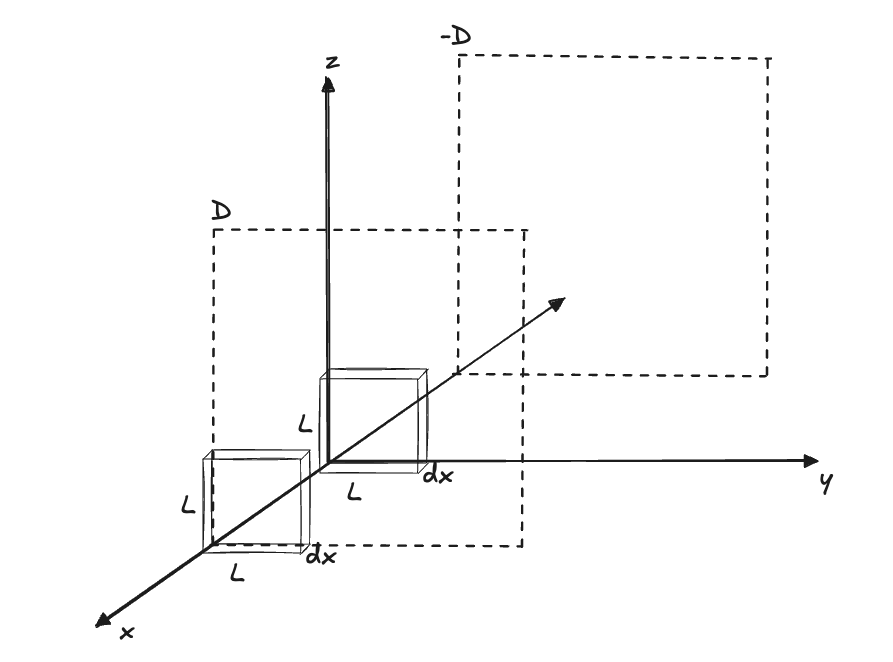
\includegraphics[scale=0.3]{ch2-12.png}
    \end{center}
    \begin{itemize}
        \item [(a)] We want to compute first the electric field when
        $-D < x < D$. Let us consider a differential volume $dV = l^2dx$
        between $-D$ and $D$ then the electric field on the volume must be in
        the $x$ direction by symmetry.
        The charge inside this differential volume is
        \begin{align*}
            dQ = \rho l^2 dx
        \end{align*}
        Hence by integration we get that
        \begin{align*}
            Q = \int_0^x \rho l^2 dx = \rho l^2 x
        \end{align*}
        Now to solve $\int E\cdot dS$ we see that only the front and back faces
        of the volume contribute to the integral so $\int E\cdot dS = 2E_x l^2$
        therefore by Gauss' law we have that
        \begin{align*}
            2E_x l^2 &= 4\pi(2\rho l^2 x)\\
            E_x &= 4\pi \rho x
        \end{align*}
        Where we also used that to account for the charge on the section from
        0 to $-D$ we need to muliply $Q$ by $2$.

        To compute the electric field at $x \geq D$ we consider another
        differential volume placed at $x = D$ as shown in the figure. Then
        the charge inside this differential volume is
        \begin{align*}
            dQ = \rho l^2 dx
        \end{align*}
        And hence by integration we get that
        \begin{align*}
            Q = \int_0^D \rho l^2 dx = \rho l^2 D
        \end{align*}
        Again the front and back faces are the only ones that contribute to
        the electrical field so by Gauss' law we have that
        \begin{align*}
            2E_x l^2 &= 4\pi(2\rho l^2 D)\\
            E_x &= 4\pi \rho D
        \end{align*}
        Finally, for a differential volume placed at $x=-D$ what changes is
        the integration of $dQ$ where we integrate from $0$ to $-D$ to obtain
        the following
        \begin{align*}
            Q = \int_0^{-D} \rho l^2 dx = -\rho l^2 D
        \end{align*}
        Theferore in this case, we get that 
        \begin{align*}
            E_x &= -4\pi \rho D
        \end{align*}

        \item [(b)] We know that the electrostatic potential is given by
        \begin{align*}
            \bm{\phi(x)} = - \int_{x_0}^x \bm{E(x') \cdot dx'}
        \end{align*}
        where $x_0$ is some reference point. So taking $x_0 = -D$ and $x = D$
        to get the potential difference between these points we can write that
        \begin{align*}
            \phi(x) &= - \int_{-D}^D 4\pi\rho x~dx \\
            &= -4\pi\rho \bigg[\frac{D^2}{2} - \frac{(-D)^2}{2}\bigg]\\
            &= 0
        \end{align*}
    \end{itemize}
\end{proof}
\cleardoublepage
\begin{proof}{\textbf{14.}}
    Let us consider the following section of the cylinder described
    \begin{center}
        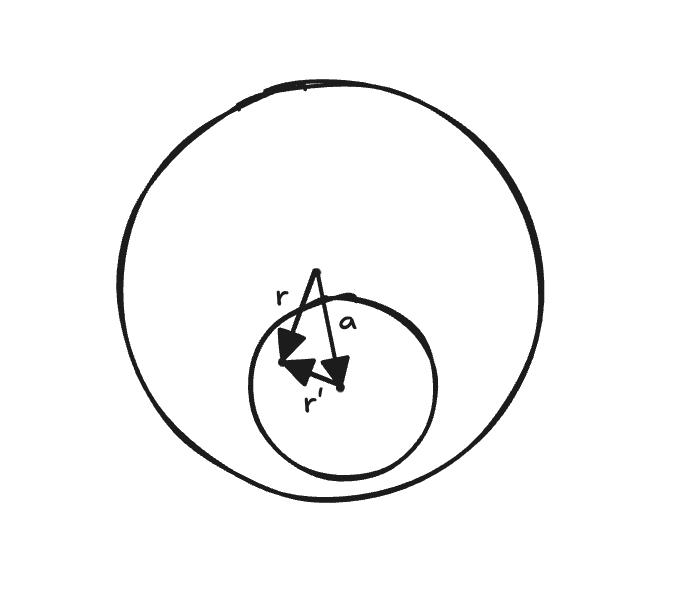
\includegraphics[scale=0.3]{ch2-14.png}
    \end{center}
    Assuming the cylindrical cavity doesn't exists.
    Let us consider a point at a distance $\bm r$ from the center of the big
    cylinder of radius $R$ then the electric field at this point will be in the
    direction of $\bm{r}$ and we can determine the magnitude of it by
    considering a cylindrical Gaussian surface of radius $r$,
    hence by Gauss' law we get that
    \begin{align*}
        \int \bm{E} \cdot d\bm{S} &= 4\pi Q\\
        E_{cyl} \cdot 2\pi r L&= 4\pi\frac{\lambda L r^2}{R^2}\\
        E_{cyl} &= \frac{2\lambda r}{R^2}
    \end{align*}
    Where we used that the charge enclosed by the Gaussian surface is
    $\lambda L r^2/R^2$. In vector form we get that
    \begin{align*}
        \bm E_{cyl} &= \frac{2\lambda r}{R^2} \hatr = \frac{2\lambda}{R^2} \bm{r}
    \end{align*}
    Now if we consider the same point but from the cavity's centre,
    assuming the cavity has a charge $-\lambda L r'^2/R^2$ the electric field
    is given by
    \begin{align*}
        E_{hole} \cdot 2\pi r' L&= -4\pi \frac{\lambda L r'^2}{R^2}\\
        E_{hole} &= -\frac{2\lambda r'}{R^2}
    \end{align*}
    Or in vector form
    \begin{align*}
        \bm E_{hole} &= -\frac{2\lambda r'}{R^2} \hatr' = -\frac{2\lambda}{R^2} \bm{r'}
    \end{align*}
    Therefore the total electric field is the sum of both electric fields i.e. 
    \begin{align*}
        \bm E &= \bm E_{cyl} + \bm E_{hole}\\
        \bm E &= \frac{2\lambda}{R^2} \bm{r} - \frac{2\lambda}{R^2} \bm{r'}\\
        \bm E &= \frac{2\lambda}{R^2} \bm{a}        
    \end{align*}
    Where $\bm{a}$ is the distance from the big cylinder centre to the cavity's
    centre.
\end{proof}
\cleardoublepage
\begin{proof}{\textbf{15.}}
    Lets first compute the electric field inside the cylinder using Gauss'
    law
    \begin{align*}
        \int \bm{E}\cdot d\bm{S} &= 4\pi Q\\
        E_{inside} \cdot 2\pi r L &= 4\pi \frac{\lambda Lr^2}{R_1^2}\\
        E_{inside} &= \frac{2\lambda r}{R_1^2}
    \end{align*}
    Also, the electric field in the space between the cylinder and the shell is 
    \begin{align*}
        \int \bm{E}\cdot d\bm{S} &= 4\pi Q\\
        E_{outside} \cdot 2\pi r L &= 4\pi \lambda L\\
        E_{outside} &= \frac{2\lambda}{r}
    \end{align*} 
    Since the enclosed charge is the charge of the cylinder.  
    Now we determine the electrostatic potential using
    \begin{align*}
        \Phi(\bm{x}) = - \int_{x_0}^x E(\bm{x}')\cdot d\bm{x}'
    \end{align*}
    Hence
    \begin{align*}
        \Phi(r)
        &= -\bigg[\int_{0}^{R_1} \frac{2\lambda r}{R_1^2} dr
        + \int_{R_1}^{R_2} \frac{2\lambda}{r} dr \bigg] \\
        &= -\bigg[\frac{2\lambda}{R_1^2}\frac{R_1^2}{2}
        + 2\lambda\log(\frac{R_2}{R_1}) \bigg] \\
        &= -\lambda + 2\lambda\log(\frac{R_1}{R_2})\\
        &= \lambda \bigg(2\log(\frac{R_1}{R_2}) - 1\bigg)
    \end{align*}
\end{proof}
\cleardoublepage
\begin{proof}{\textbf{19.}}
    Let us consider a point at a distance $d$ from the center of the cylinder
    as shown below
    \begin{center}
        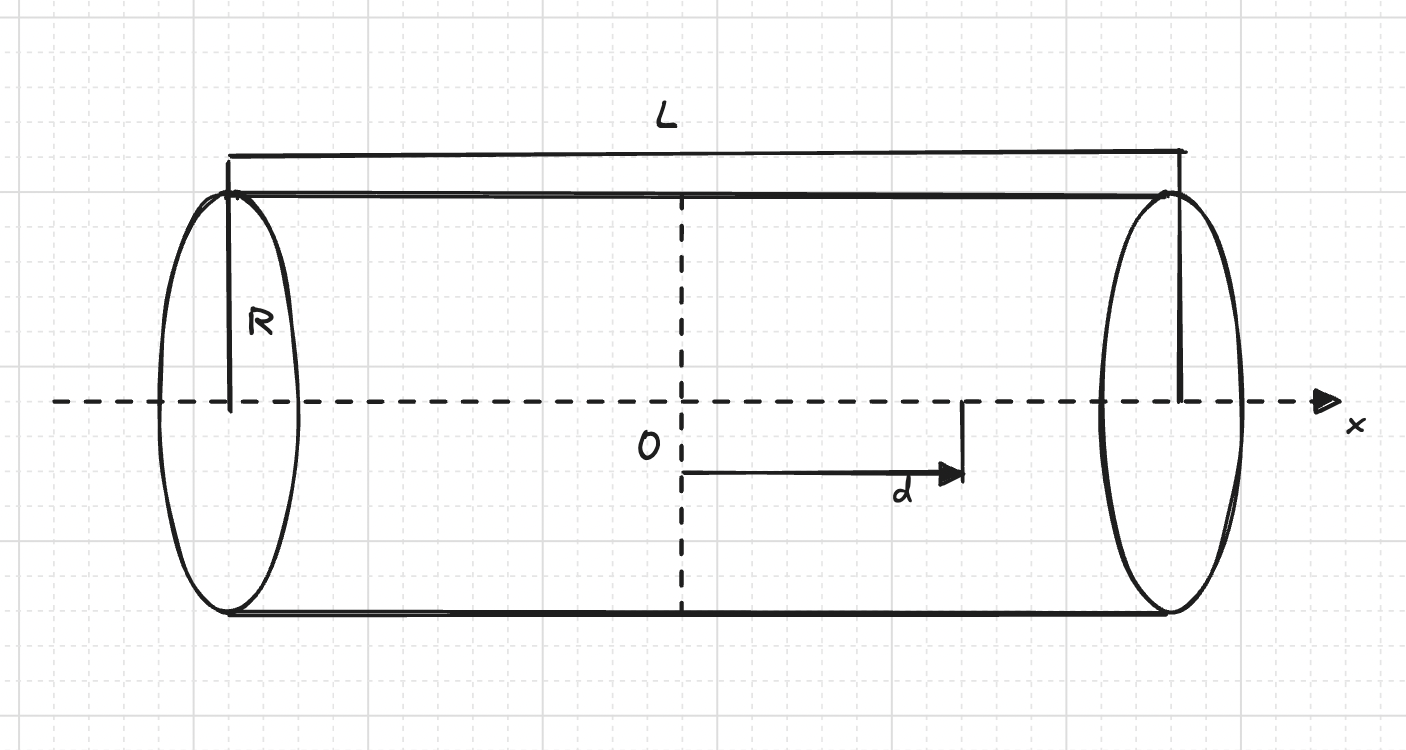
\includegraphics[scale=0.4]{ch2-19.png}
    \end{center}    
    Lets consider a small piece in cylindrical coordinates $r'dr'd\phi'dx'$.
    Since the charge per unit of volume is $Q/\pi R^2 L$
    then the electric field because of this small piece at a distance $d$
    from the center is
    \begin{align*}
        dE = \frac{Qr'dr'd\phi'dx'}{\pi R^2 L} \frac{1}{(d - x')^2 + r'^2}
    \end{align*}
    But because of the symmetry the only component we care about is the 
    horizontal component in the $x$ direction hence
    \begin{align*}
        dE_x
        &= \frac{Qr'dr'd\phi'dx'}{\pi R^2 L}
        \frac{1}{(d - x')^2 + r'^2} \cos\theta\\
        &= \frac{Qr'dr'd\phi'dx'}{\pi R^2 L}
        \frac{1}{(d - x')^2 + r'^2}\frac{d-x'}{\sqrt{(d - x')^2 + r'^2}}\\
        &= \frac{Qr'dr'd\phi'dx'}{\pi R^2 L}
        \frac{d-x'}{((d - x')^2 + r'^2)^{3/2}}
    \end{align*}
    Then by integration we have that
    \begin{align*}
        E_x &= \frac{Q}{\pi R^2 L}\int_{-L/2}^{L/2}\int_0^{2\pi}\int_0^R
        \frac{(d-x')r'}{((d - x')^2 + r'^2)^{3/2}} dr'd\phi'dx'\\
        &= \frac{Q}{\pi R^2 L}\int_{-L/2}^{L/2}\int_0^{2\pi}
        \bigg[\frac{1}{(d-x')}-\frac{1}{\sqrt{(d-x')^2 + R^2}}\bigg]
        (d-x')d\phi'dx'\\
        &= \frac{2Q}{R^2 L}\int_{-L/2}^{L/2}
        \bigg[1-\frac{(d-x')}{\sqrt{(d-x')^2 + R^2}}\bigg]
        dx'\\
        &= \frac{2Q}{R^2 L}\bigg[
            L + \sqrt{(d-L/2)^2 + R^2} - \sqrt{(d+L/2)^2 + R^2} 
        \bigg]
    \end{align*}
    Now we compute the electrostatic potential as follows
    \begin{align*}
        \Phi &= \frac{2Q}{R^2 L}\int_0^d 
        L + \sqrt{(x'-L/2)^2 + R^2} - \sqrt{(x'+L/2)^2 + R^2}~dx'\\
        &= \frac{2Q}{R^2 L}
        \bigg[
            \frac{1}{2}
            \bigg[ 2Lx' + (x'-L)\sqrt{(x'-L/2)^2 + R^2}
            - (x'+L)\sqrt{(x'+L/2)^2 + R^2}\\
            &\quad-R^2\text{arctanh}\bigg(
                \frac{L-x'}{\sqrt{(x'-L/2)^2 + R^2}}
            \bigg)
            -R^2\text{arctanh}\bigg(
                \frac{L+x'}{\sqrt{(x'+L/2)^2 + R^2}}
            \bigg)
        \bigg]\bigg]_0^d\\
        &= \frac{2Q}{R^2 L}
        \bigg[
            \frac{1}{2}
            \bigg[
            2Ld + (d-L)\sqrt{(d-L/2)^2 + R^2}
        - (d+L)\sqrt{(d+L/2)^2 + R^2}\\
        &\quad-R^2\text{arctanh}\bigg(
                \frac{L-d}{\sqrt{(d-L/2)^2 + R^2}}
            \bigg)
        -R^2\text{arctanh}\bigg(
                \frac{L+d}{\sqrt{(d+L/2)^2 + R^2}}
            \bigg)
        \bigg]\\
        &-\frac{1}{2}
        \bigg[
            -L\sqrt{L^2/4 + R^2}
            - L\sqrt{L^2/4 + R^2}
            -2R^2\text{arctanh}\bigg(\frac{L}{\sqrt{L^2/4 + R^2}}\bigg)
        \bigg]
        \bigg]
    \end{align*}

\end{proof}
\cleardoublepage
\begin{proof}{\textbf{20.}}
    \begin{itemize}
        \item [(a)] Let us consider a spherical Gaussian surface enclosing
        the spherically symmetric charge, then $\bm{E} = E\hatr$ and hence by
        Gauss' law we have that
        \begin{align*}
            \int_{0}^{2\pi}\int_{0}^{\pi} E~r^2\sin\theta d\theta d\phi
            &= 4\pi\int_{0}^{2\pi}\int_{0}^{\pi}\int_{0}^{r}
            \rho~r^2\sin\theta d\theta d\phi dr\\
            4\pi Er^2 &= 
            4\pi k\int_{0}^{2\pi}\int_{0}^{\pi}\int_{0}^{r}
            r^n~r^2\sin\theta d\theta d\phi dr\\
            Er^2 &= 4\pi k\int_{0}^{r} r^{n + 2} dr
        \end{align*}
        We know that $n > -3$ then $n + 2 \geq 0$ so knowing this we can solve
        the integral as follows
        \begin{align*}
            Er^2 &= 4\pi k~\frac{r^{n + 3}}{n+3}\\
            E &= 4\pi k~\frac{r^{n + 1}}{n+3}
        \end{align*}

        \item [(b)] To find the potential difference between the points
        $r = a$ and $r = b$ we solve the following integral
        \begin{align*}
            \Phi(r) = - \int_a^b E(r) dr
        \end{align*}
        Since $E$ only depends on $r$ hence
        \begin{align*}
            \Phi(r) &= - 4\pi k \int_a^b \frac{r^{n + 1}}{n+3}~dr\\
                &= - \frac{4\pi k}{n+3} \int_a^b r^{n + 1}~dr
        \end{align*}
        Therefore
        \begin{align*}
            \Phi(r) &= \begin{cases}
                - \frac{4\pi k}{n+3} \log(\frac{b}{a}) &\text{ if }n = -2\\
                - \frac{4\pi k}{(n+3)(n+2)}[b^{n+2} - a^{n+2}]
                &\text{ if }n \geq -1\\
            \end{cases}
        \end{align*}
    \end{itemize}
\end{proof}
\cleardoublepage
\begin{proof}{\textbf{21.}}
    Let the potential in some region be
    \begin{align*}
        \Phi(x,y,z) = ax^2 + by^3
    \end{align*}
    By the Poisson's equation we know that
    \begin{align*}
        \laplacian{\Phi(\bm{x})} = -4\pi \rho(\bm{x})
    \end{align*}
    Then the charge density is given by
    \begin{align*}
        -4\pi \rho(x,y,z)
        &= \partialderivative[2]{\Phi}{x} + \partialderivative[2]{\Phi}{y} +
        \partialderivative[2]{\Phi}{z}\\
        \rho(x,y,z)
        &= -\frac{1}{4\pi}\big(2a + 6by\big) 
    \end{align*}
\end{proof}
\cleardoublepage
\begin{proof}{\textbf{23.}}
    From the hint we have we can compute the following
    \begin{align*}
        \derivative{r}{\theta} &= \frac{E_r}{E_\theta}\\
        &= \frac{2pr^3\cos\theta}{pr^3\sin\theta}\\
        &= \frac{2\cos\theta}{\sin\theta}\\
        &= 2\cot\theta
    \end{align*}
    Hence by integration
    \begin{align*}
        \int dr &= 2\int \cot\theta~d\theta\\
        r &= 2\log(\sin\theta) + C
    \end{align*}
    Which is the polar equation for the electric field lines. 
\end{proof}
\cleardoublepage
\begin{proof}{\textbf{25.}}
    \begin{itemize}
        \item [(a)] According to equation (61) the force that a point charge
        $q'$ exerts on a dipole of moment $p$ is
        \begin{align*}
            \bm{F} = (\bm{p}\cdot\nabla) \bm{E}(\bm{x})
        \end{align*}
        A point charge $q'$ produces an electric field
        $\bm{E}(r) = q'\frac{\bm{r}}{|\bm{r}|^3}$ then
        \begin{align*}
            \bm{F} &= p(\hatz\cdot\nabla) q'\frac{\bm{r}}{|\bm{r}|^3}\\
            &= p\pdv{z}(q'\frac{\rho\hatrho + z\hatz}{(\rho^2 + z^2)^{3/2}})\\
            &= pq'\left[-\frac{3z\rho}{(\rho^2 + z^2)^{5/2}}\hatrho
            + \frac{\rho^2 - 2z^2}{(\rho^2 + z^2)^{5/2}}\hatz\right]
        \end{align*}
        But given that the charge is in the $x$-$y$ plane we can set
        $z=0$ hence
        \begin{align*}
            \bm{F} &= \frac{pq'}{\rho^3}\hatz       
        \end{align*}

        \item [(b)] According to Coulomb's law the force a dipole exerts on
        a point charge $q'$ is 
        \begin{align*}
            \bm{F} = q'\bm{E}
        \end{align*}
        Where $\bm{E}$ is the electric field produced by the dipole, hence
        \begin{align*}
            \bm{F} = q'\left(
                2p\frac{\cos\theta}{\rho^3}\hatrho
                + p\frac{\sin\theta}{\rho^3}\hattheta
            \right)
        \end{align*}
        But cosidering that the charge is in the $x$-$y$ plane we have that
        $\theta = \pi/2$ hence
        \begin{align*}
            \bm{F} = \frac{pq'}{\rho^3}\hattheta
        \end{align*}
        Also, in this position the spherical unit vector $\hattheta$
        matches with the rectangular unit vector $-\hatz$
        therefore 
        \begin{align*}
            \bm{F} = -\frac{pq'}{\rho^3}\hatz
        \end{align*}
        Which is in agreement with Newton's Third Law.
    \end{itemize}
\end{proof}
\cleardoublepage
\begin{proof}{\textbf{26.}}
    According to the equation (65) the torque that a point charge $q'$ exerts
    on a dipole of moment $p$ is
    \begin{align*}
        \bm{\tau} = \bm{p} \times \bm{E}
    \end{align*}
    Where $\bm{E}$ is the electric field generated by $q'$. Hence in
    cylindrical coordinates we have that
    \begin{align*}
        \bm{\tau} &= p\hatz \times q'\frac{\rho\hatrho + z\hatz}{(\rho^2 + z^2)^{3/2}}\\
        &= \frac{pq'\rho}{(\rho^2 + z^2)^{3/2}}\hattheta
    \end{align*}
    But if we change to spherical coordinates we get that
    \begin{align*}
        \bm{\tau} &= \frac{pq'\sin\theta}{r^2}\hatphi
    \end{align*}
    Where we used that $r^2 = (\rho^2 + z^2)$ and that $\hattheta = \hatphi$.
 
    On the other hand, from problem 25 we know that the force a dipole exerts
    on a point charge in spherical coordinates is
    \begin{align*}
        \bm{F} = q'\left(
            2p\frac{\cos\theta}{r^3}\hatr
            + p\frac{\sin\theta}{r^3}\hattheta
        \right)
    \end{align*}
    Then the torque exerted by the dipole on the point charge is
    \begin{align*}
        \bm{\tau} &= \bm{r} \times \bm{F}\\
        &= r\hatr \times q'\left(
            2p\frac{\cos\theta}{r^3}\hatr
            + p\frac{\sin\theta}{r^3}\hattheta
        \right)\\
        &= \frac{pq'\sin\theta}{r^2}\hatphi
    \end{align*}
\end{proof}
\cleardoublepage
\begin{proof}{\textbf{28.}}
    We know by definition that
    \begin{align*}
        E_x = -\pdv{\Phi}{x} \qquad E_y = -\pdv{\Phi}{y} \qquad E_z = -\pdv{\Phi}{z}
    \end{align*}
    Then 
    \begin{align*}
        \laplacian E_x &= \laplacian \left(-\pdv{\Phi}{x}\right)\\
        &= -\left[\pdv[2]{x}\pdv{\Phi}{x} + \pdv[2]{y}\pdv{\Phi}{x}
        + \pdv[2]{z}\pdv{\Phi}{x}\right]\\
        &= -\left[\pdv{x}\pdv[2]{\Phi}{x} + \pdv{x}\pdv[2]{\Phi}{y}
        + \pdv{x}\pdv[2]{\Phi}{z}\right]\\
        &= -\pdv{x}\left[\pdv[2]{\Phi}{x} + \pdv[2]{\Phi}{y}
        + \pdv[2]{\Phi}{z}\right]\\
        &= -\pdv{x}\laplacian \Phi\\
        &= 0
    \end{align*}
    Where we used that $\laplacian\Phi = 0$ in a charge-free region.
    The same can be shown for $E_y$ and $E_z$.
    Hence the Mean-Value Theorem can be  applied to $E_x$, $E_y$ and $E_z$.
    The net force a spherical charge distribution experiences because of the
    electric field is
    \begin{align*}
        \bm{F} = \int_S\rho~(\uvi E_x + \uvj E_y + \uvk E_z)~dS
    \end{align*}
    But for the center applying the Mean-Value Theorem we have that
    \begin{align*}
        \bm{F} &= 4\pi r^2 \rho \left(
        \frac{\uvi}{4\pi r^2}\int_S E_x dS
        + \frac{\uvj}{4\pi r^2} \int_S E_y dS
        + \frac{\uvk}{4\pi r^2} \int_S E_z dS
        \right)\\
        &=  \rho \int_{S}(\uvi E_x + \uvj E_y + \uvk E_z) dS\\
        &=  \int_{S}\rho~(\uvi E_x + \uvj E_y + \uvk E_z) dS
    \end{align*}
    Therefore the net force experienced by the spherical distribution is as
    though all of the charge were concentrated at the center of the
    distribution.
\end{proof}
\cleardoublepage
\begin{proof}{\textbf{29.}}
    The electric field lines look like the following
    \begin{center}
        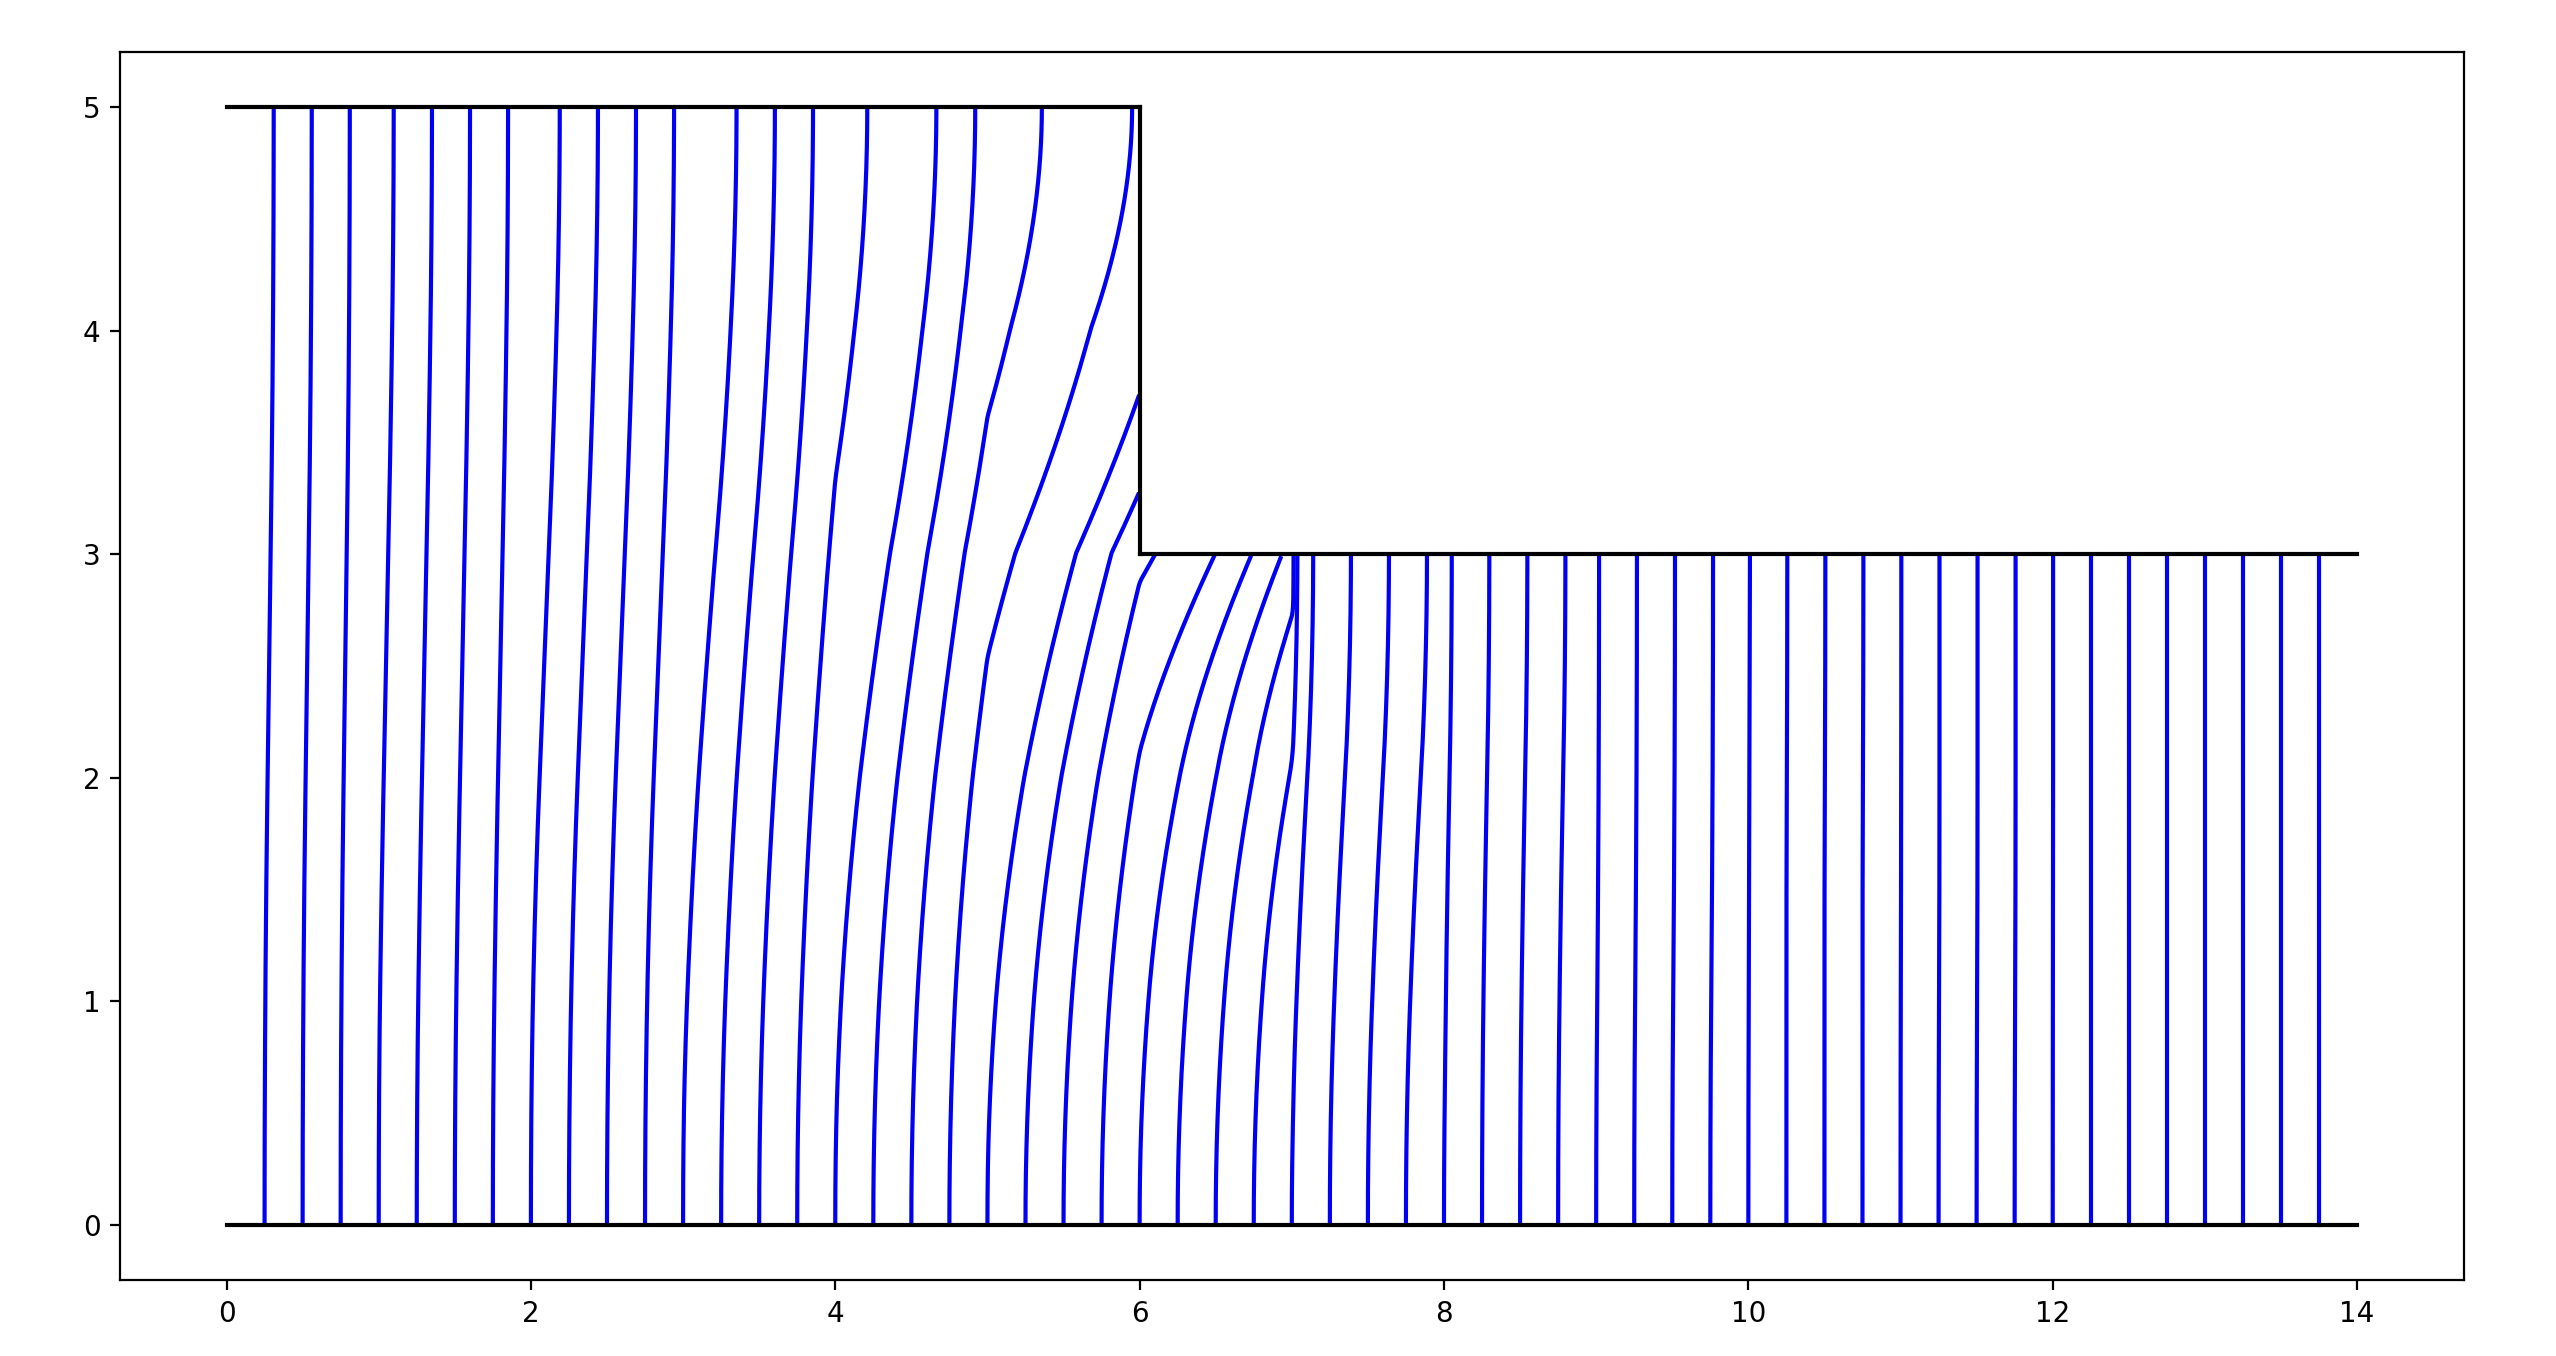
\includegraphics[scale=0.3]{ch2-29.png}
    \end{center}
    The code used to generate it is at ch2-29.py
\end{proof}
\cleardoublepage
\begin{proof}{\textbf{31.}}
    The Equipotential lines look like the following 
    \begin{center}
        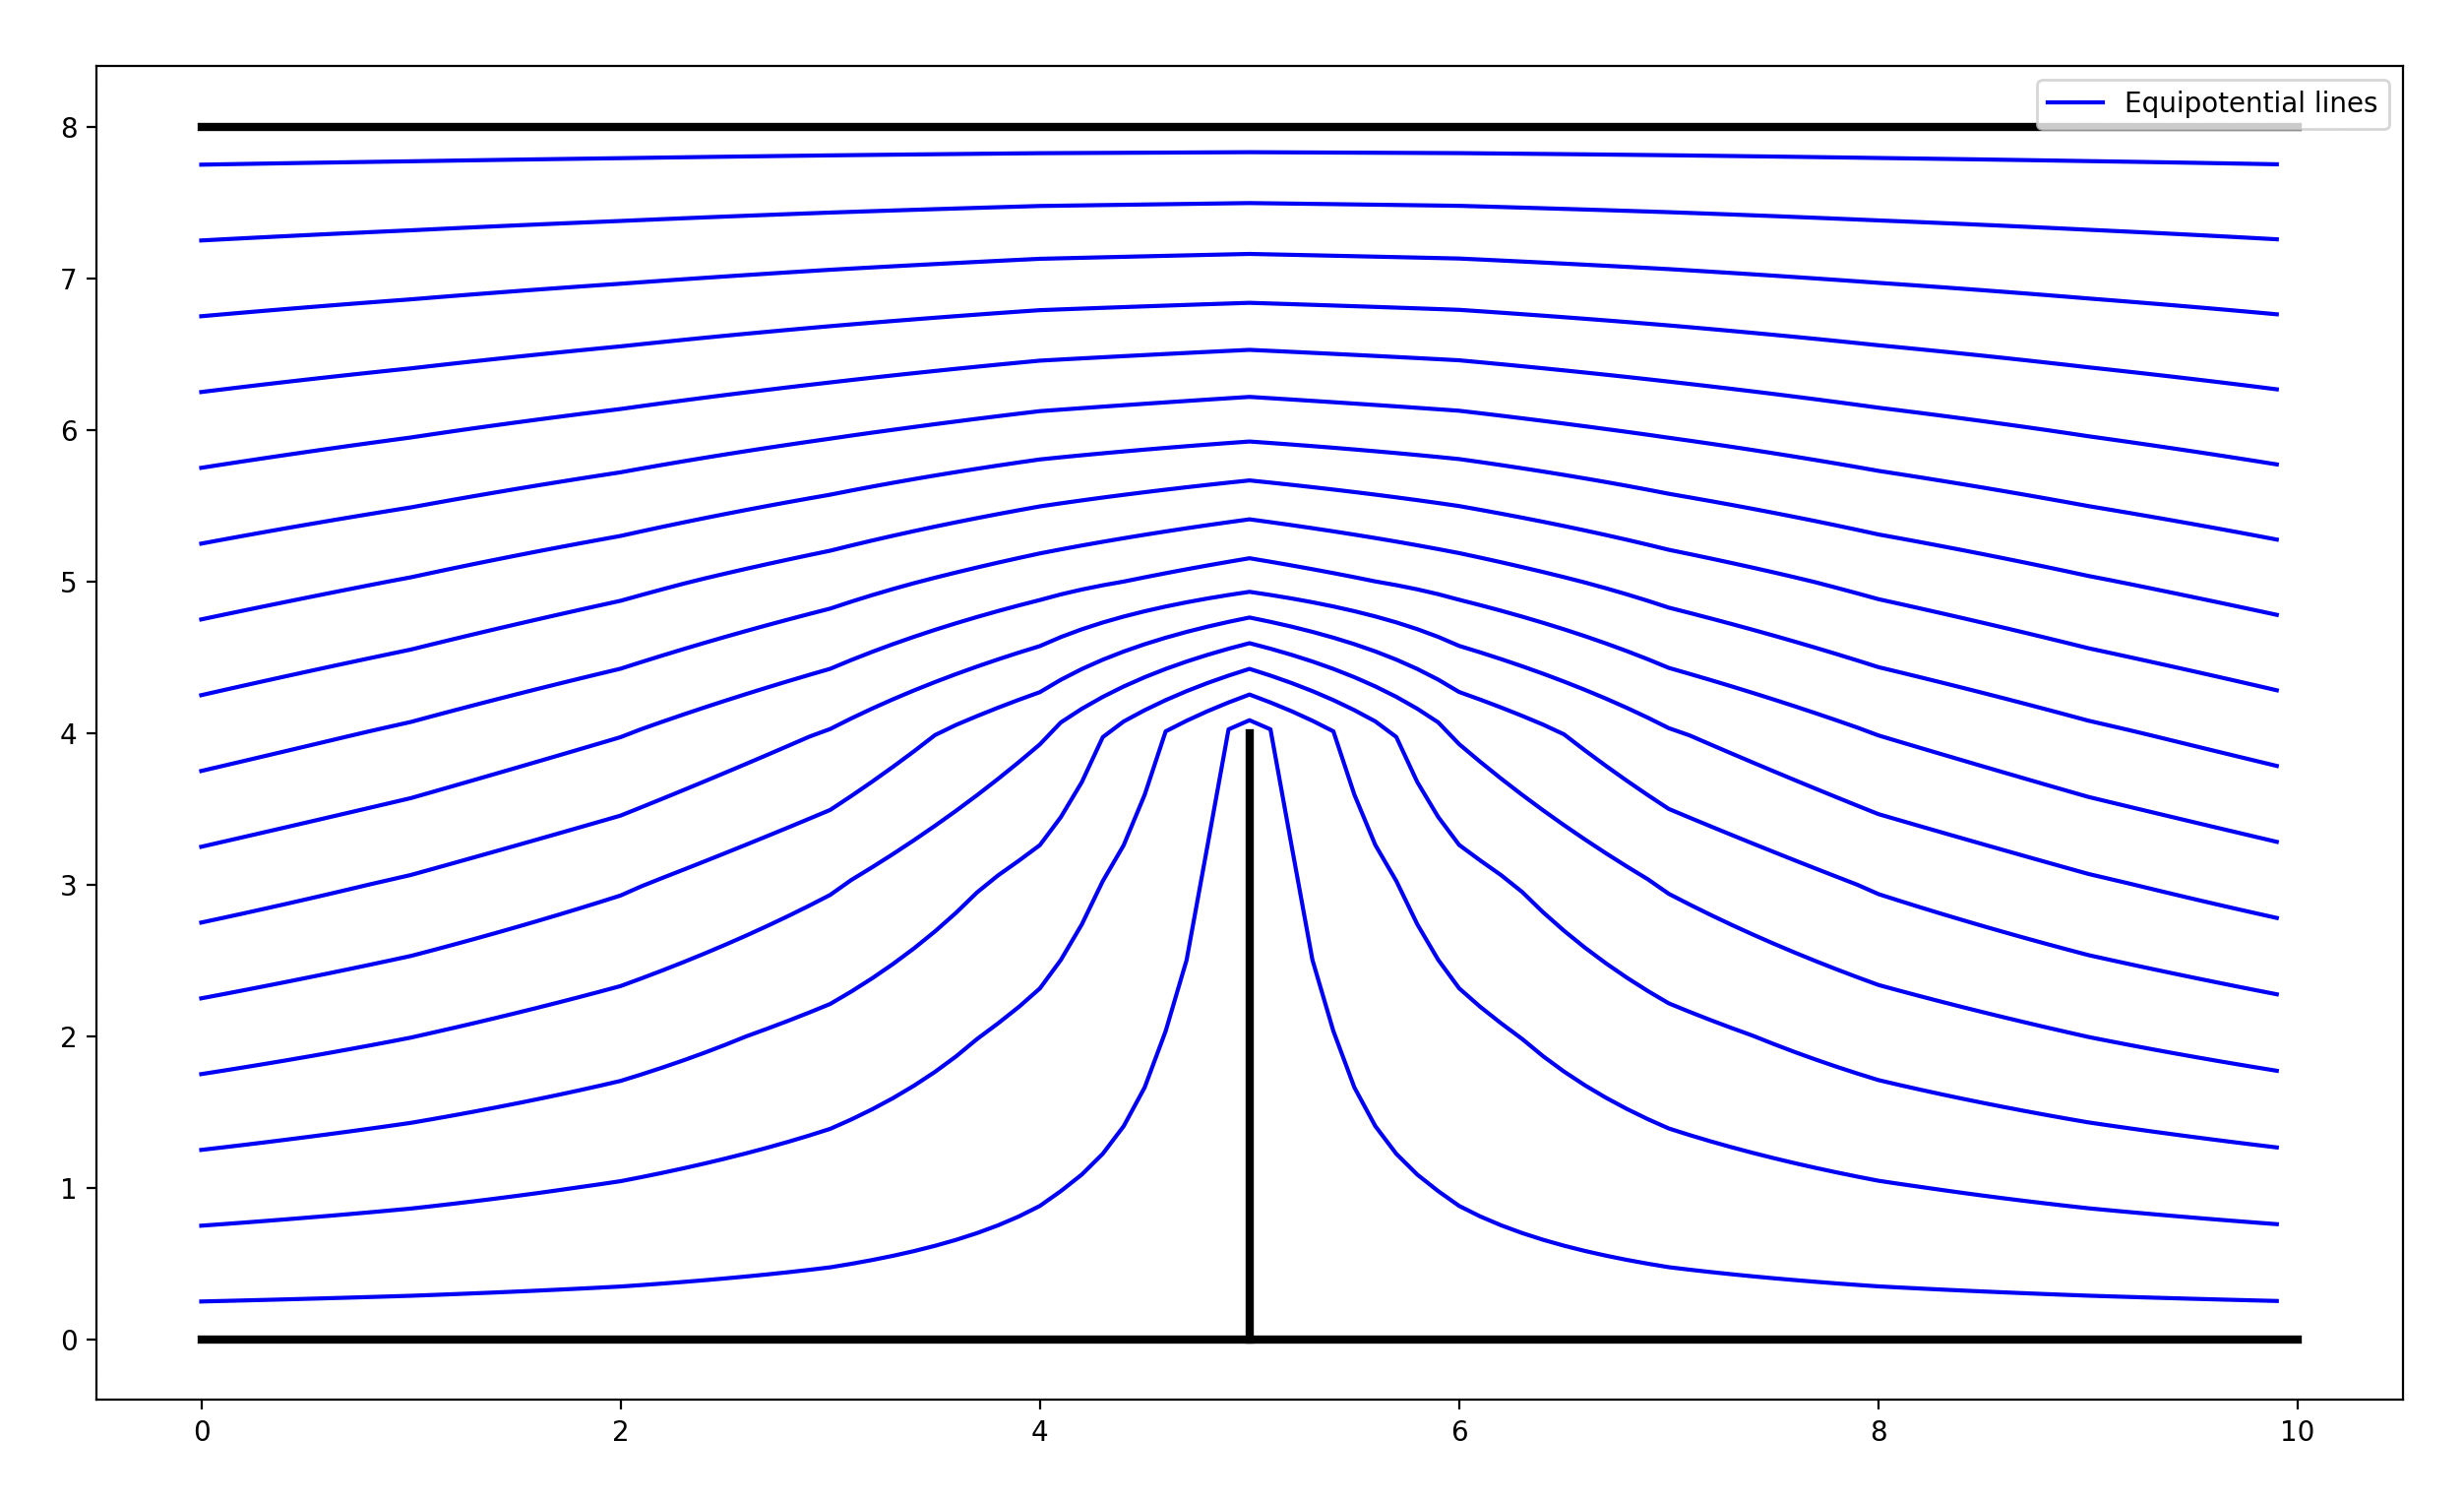
\includegraphics[scale=0.3]{ch2-31-1.png}
    \end{center}
    And the Electric field lines plus the Equipotential lines
    all together give us
    \begin{center}
        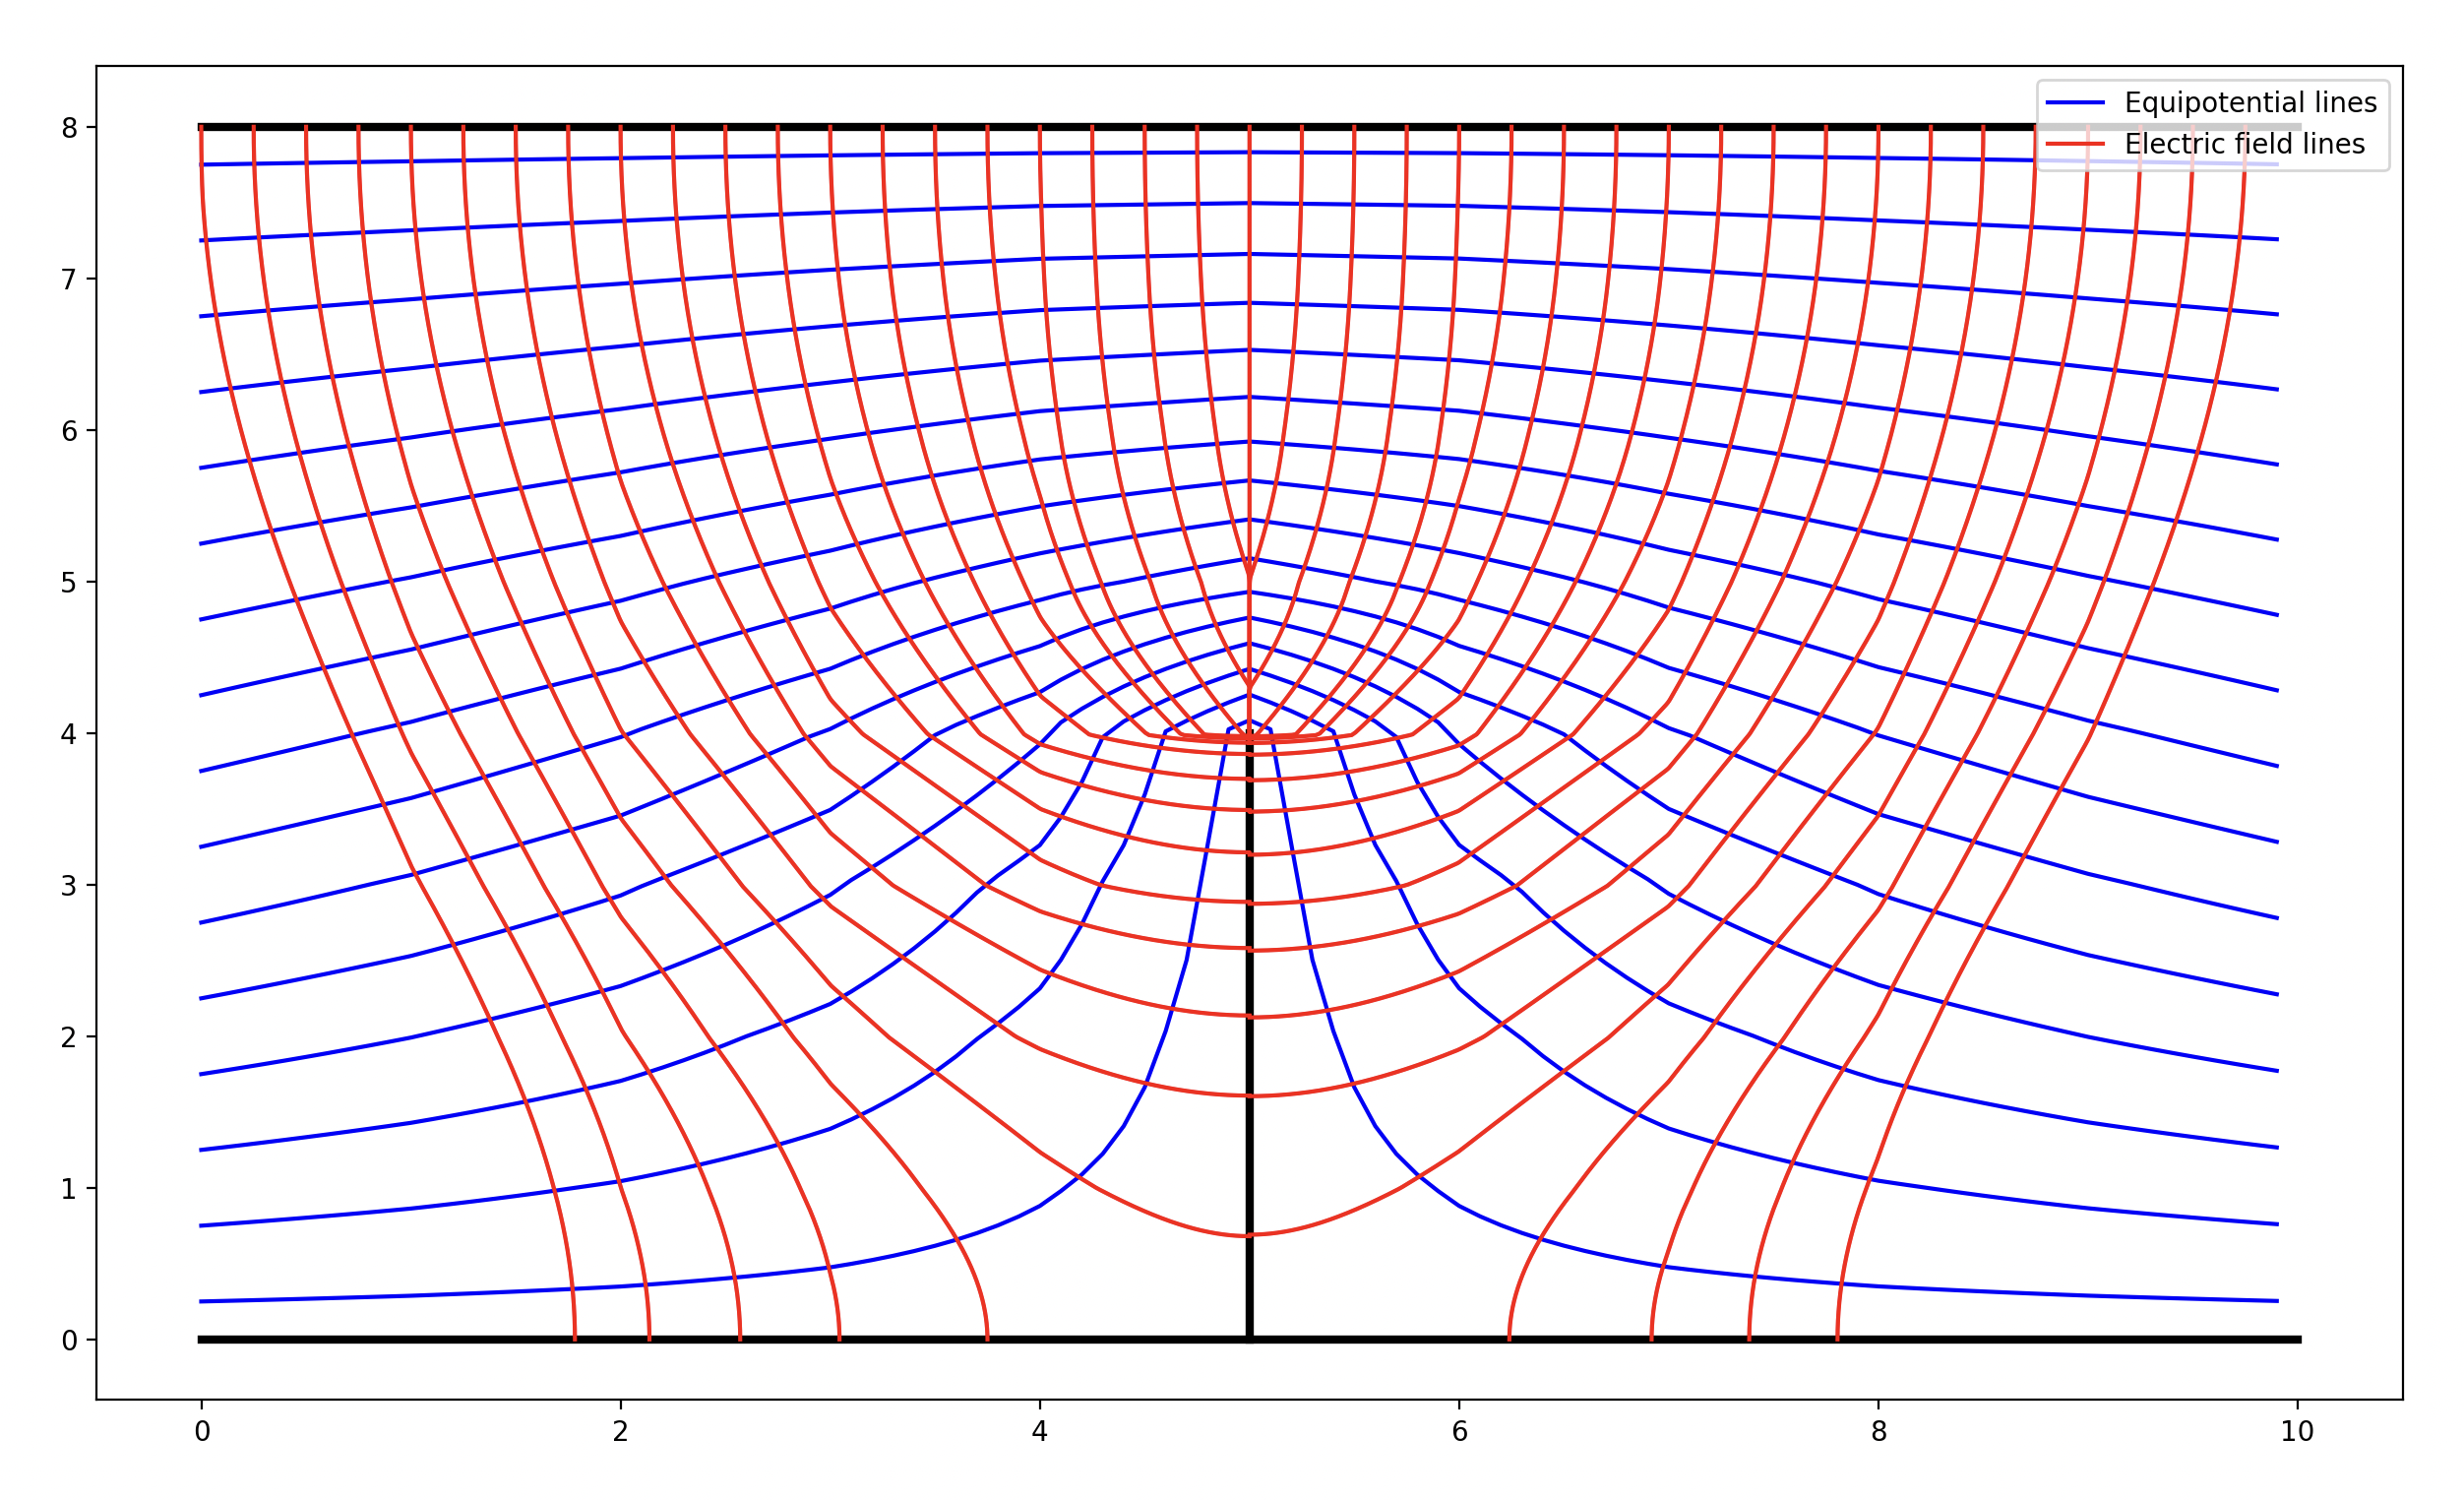
\includegraphics[scale=0.3]{ch2-31-2.png}
    \end{center}
    The code used to generate it is at ch2-31.py
\end{proof}
\cleardoublepage
\begin{proof}{\textbf{32.}}
    Equipotential lines with the original grid look like the following
    \begin{center}
        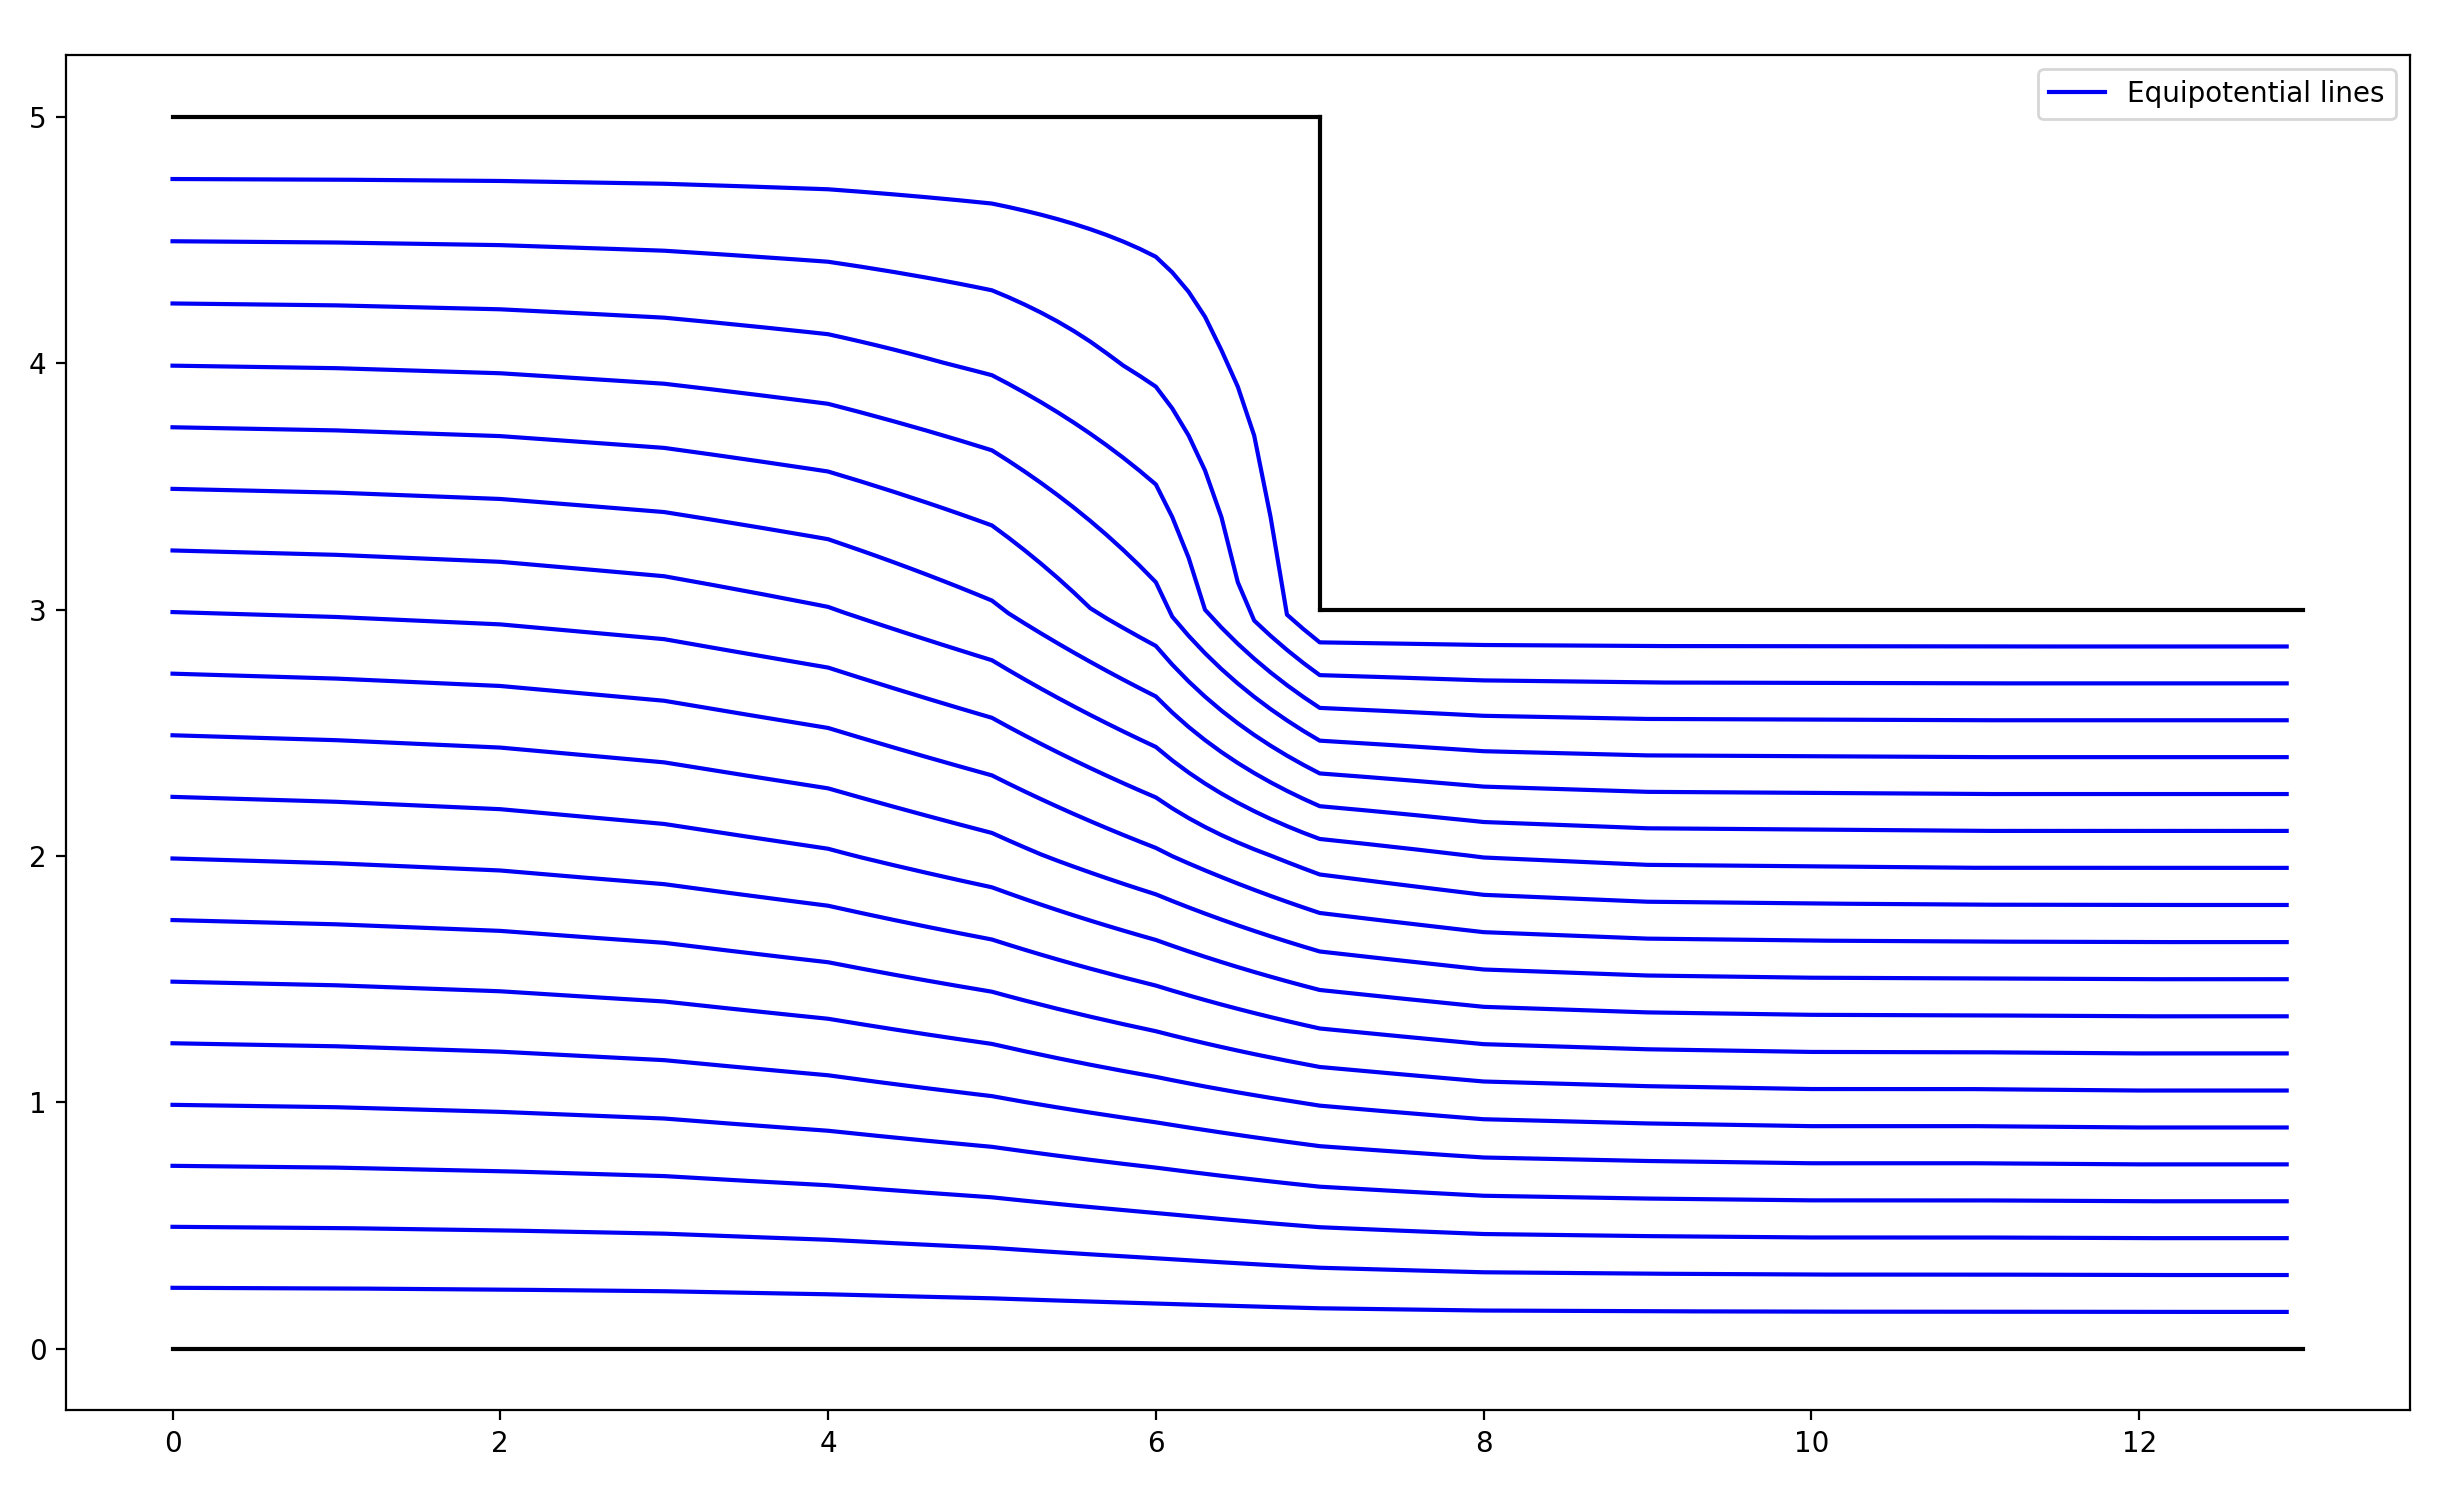
\includegraphics[scale=0.3]{ch2-32-1.png}
    \end{center}
    And with the finer grid look like the following
    \begin{center}
        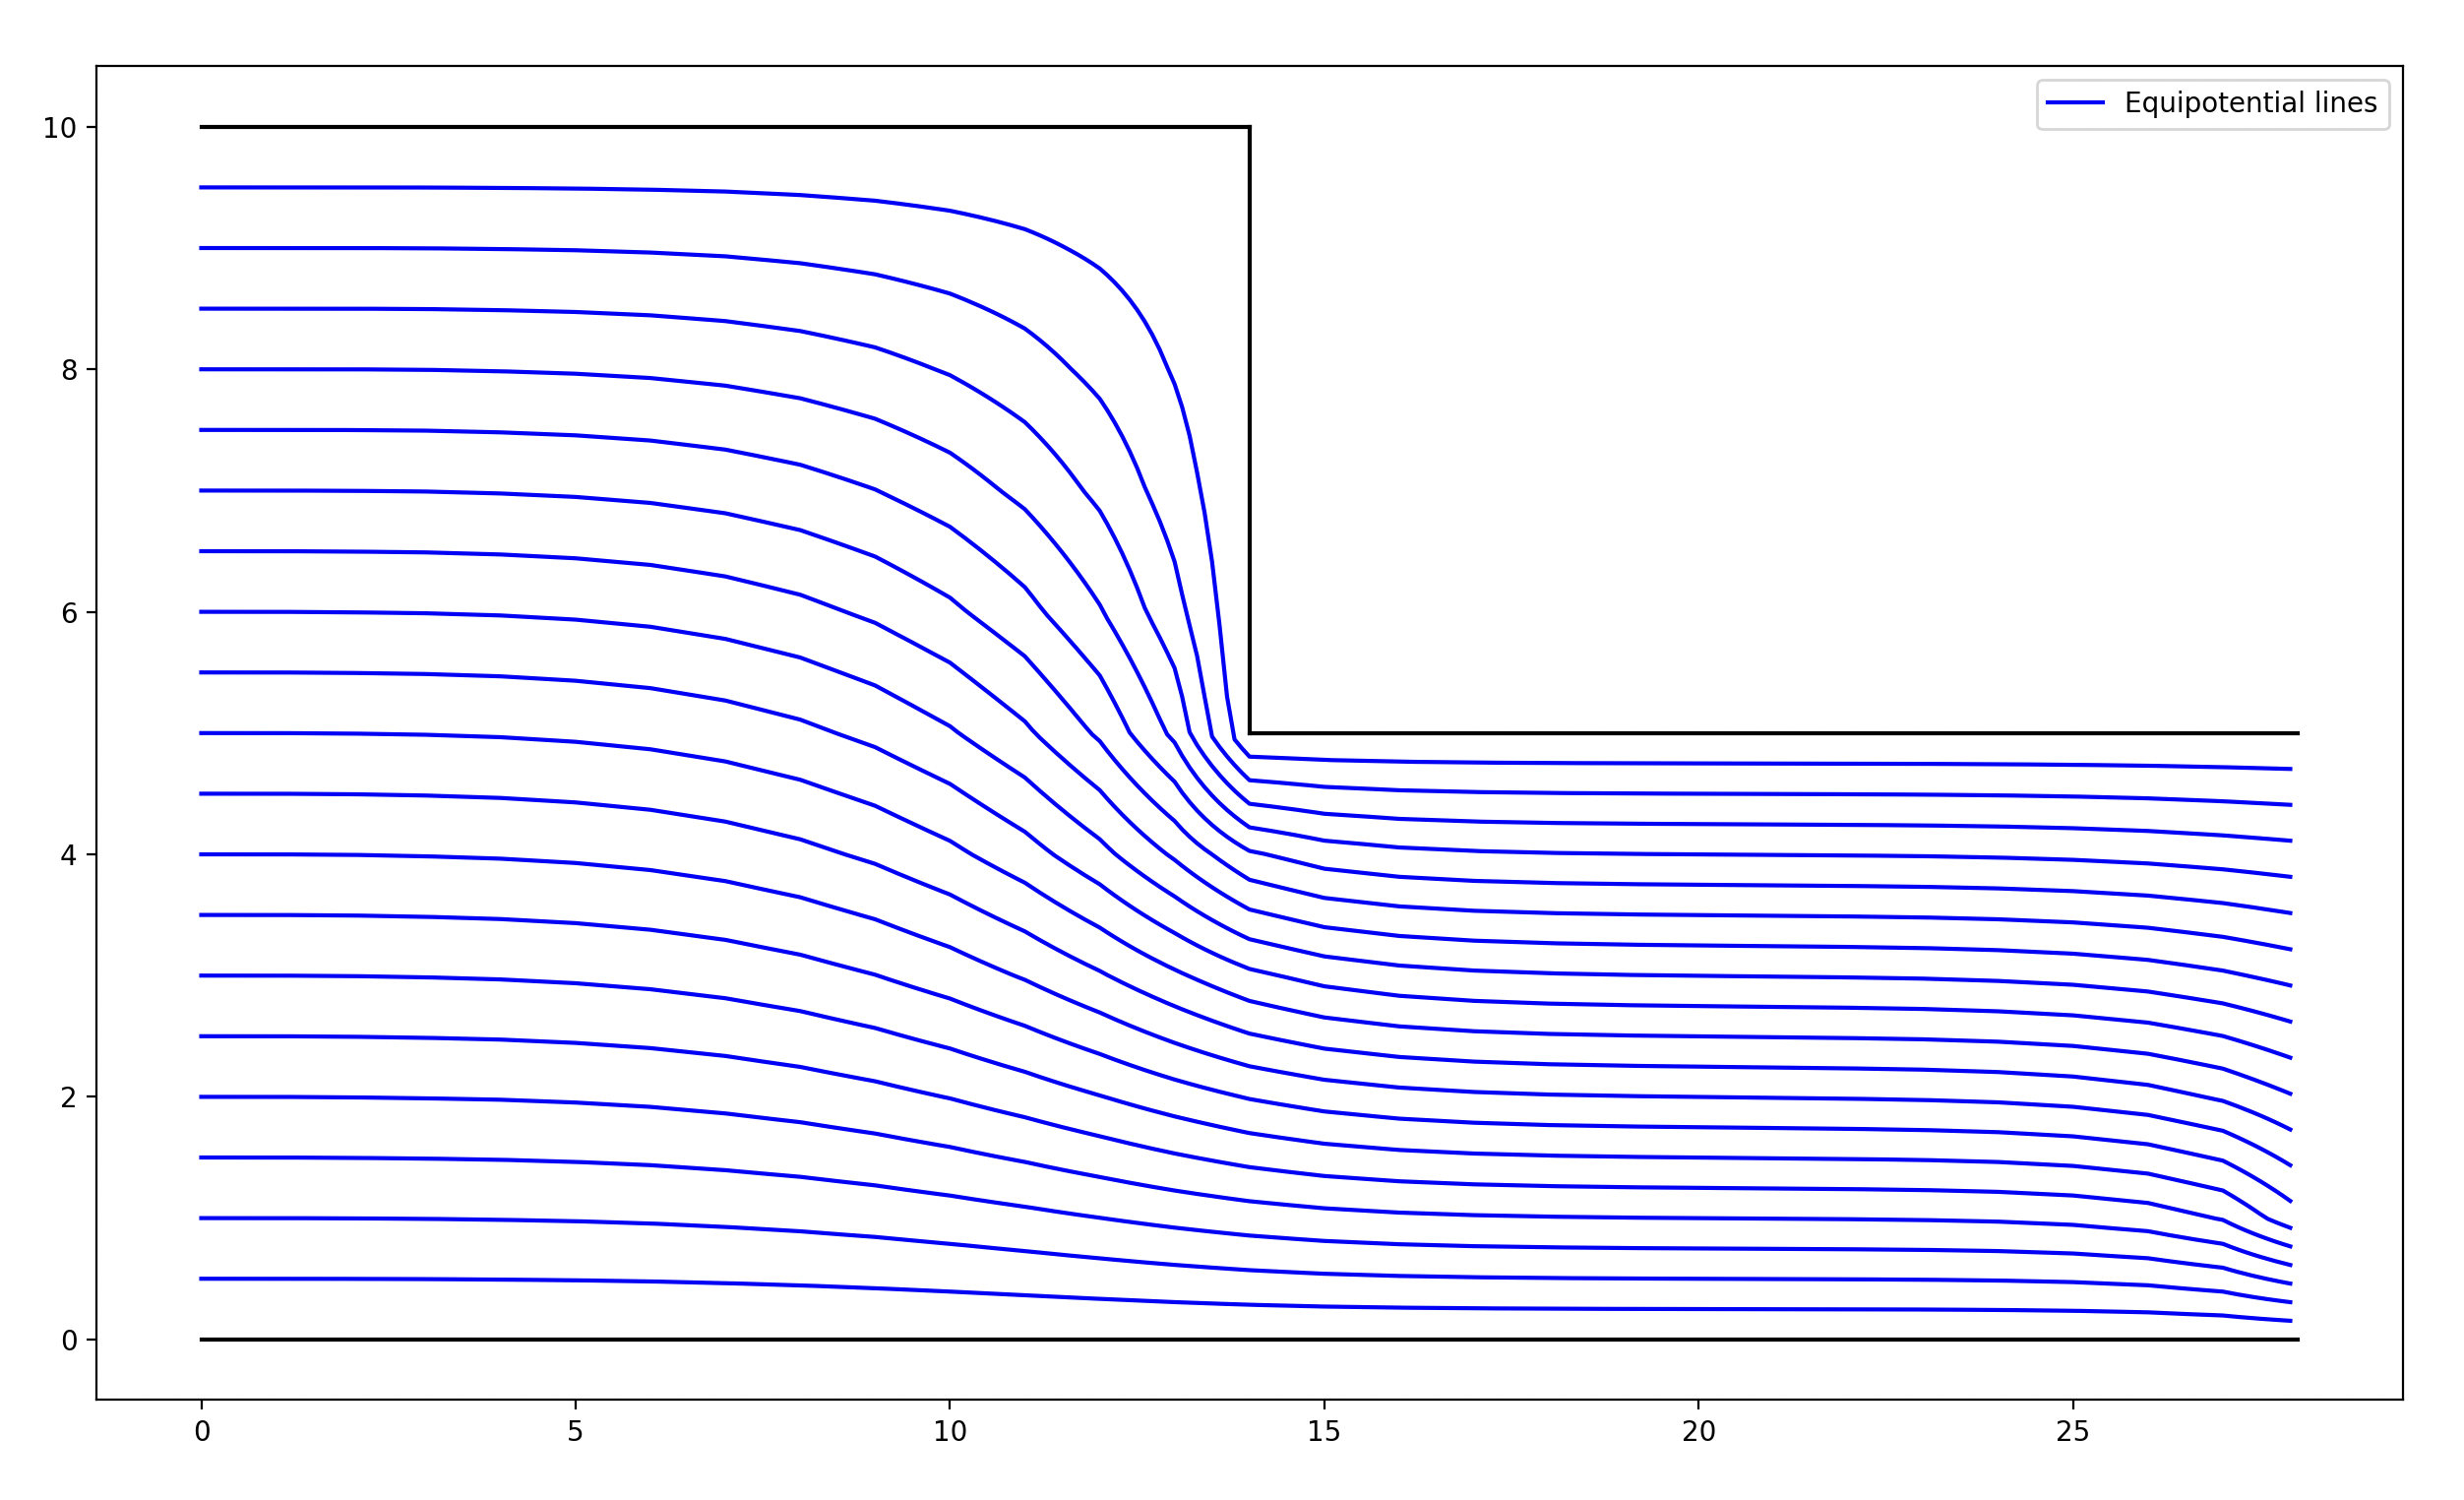
\includegraphics[scale=0.3]{ch2-32-2.png}
    \end{center}
    The code used to generate these plots is at ch2-32.py
\end{proof}
\cleardoublepage
\begin{proof}{\textbf{33.}}
    The Equipotential lines look like the following ins this case 
    \begin{center}
        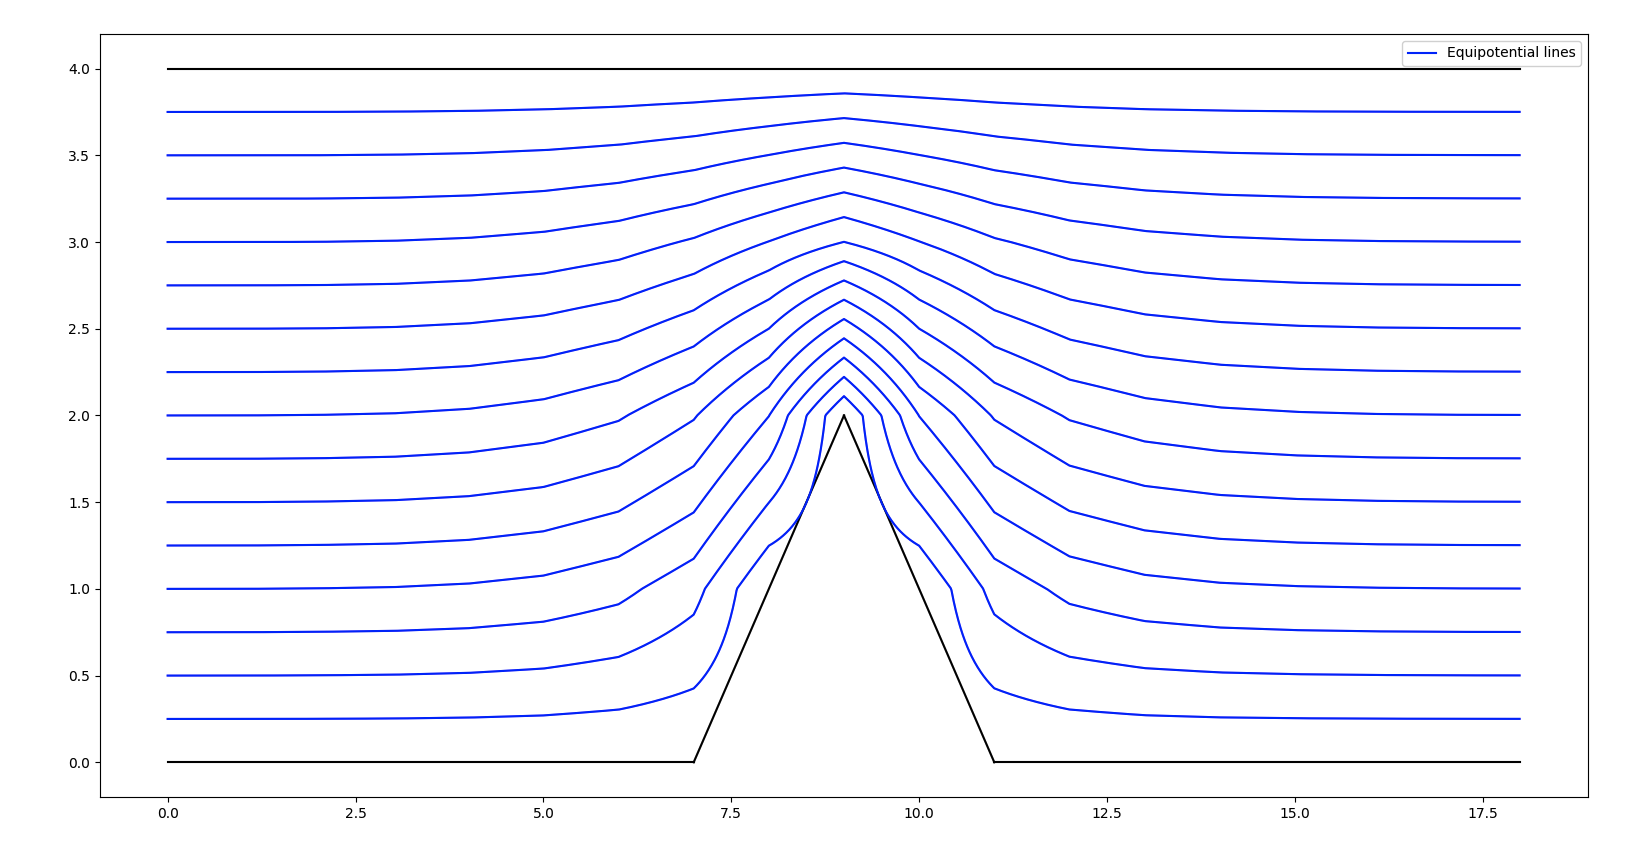
\includegraphics[scale=0.25]{ch2-33.png}
    \end{center}
    The code used to generate this plot is at ch2-33.py
\end{proof}

\end{document}
